%By% TODO: 
% - cifar10 table 
% - eig plots
% - bullet points
% - research question explicit
%Copyright (c) 2013 Joost van Zwieten
%
% Permission is hereby granted, free of charge, to any person obtaining a copy
% of this software and associated documentation files (the "Software"), to deal
% in the Software without restriction, including without limitation the rights
% to use, copy, modify, merge, publish, distribute, sublicense, and/or sell
% copies of the Software, and to permit persons to whom the Software is
% furnished to do so, subject to the following conditions:
%
% The above copyright notice and this permission notice shall be included in
% all copies or substantial portions of the Software.
%
% THE SOFTWARE IS PROVIDED "AS IS", WITHOUT WARRANTY OF ANY KIND, EXPRESS OR
% IMPLIED, INCLUDING BUT NOT LIMITED TO THE WARRANTIES OF MERCHANTABILITY,
% FITNESS FOR A PARTICULAR PURPOSE AND NONINFRINGEMENT. IN NO EVENT SHALL THE
% AUTHORS OR COPYRIGHT HOLDERS BE LIABLE FOR ANY CLAIM, DAMAGES OR OTHER
% LIABILITY, WHETHER IN AN ACTION OF CONTRACT, TORT OR OTHERWISE, ARISING FROM,
% OUT OF OR IN CONNECTION WITH THE SOFTWARE OR THE USE OR OTHER DEALINGS IN
% THE SOFTWARE.
%
\documentclass{tudelftposter}

% optional, makes QR code clickable
\usepackage[hidelinks,implicit=false,bookmarks=false]{hyperref}
\usepackage{booktabs}
\usepackage{listings}
\usepackage{xcolor}
\usepackage{mathtools}
\usepackage{subfigure}
\usepackage{subfig}

\definecolor{light-gray}{gray}{0.97} %the shade of grey that stack exchange uses
\definecolor{codegray}{rgb}{0.5,0.5,0.5}
\lstdefinestyle{mystyle}{
    language = Java,
    numberstyle=\tiny\color{codegray},
    basicstyle=\ttfamily\footnotesize,
    breakatwhitespace=false,         
    breaklines=true,                 
    captionpos=b,                    
    keepspaces=true,                 
    numbers=left,   
    numbersep=2pt,                  
    showspaces=false,                
    showstringspaces=false,
    showtabs=false,                  
    tabsize=2
}

\lstset{style=mystyle}


\title{Auto Comments: Generating Java code comments}

\addauthornote{diam}{Delft Institute of Computer Science, TU Delft}

\addauthor[diam]{R. Navin}
\addauthor[diam]{J. Katzy}
\addauthor[diam]{R. Skoulos}
\addauthor[diam]{T. Pfann}

\addfootimage(c:right column.center)[Delft Institute of Computer Science]{img/TU_P1_full-color.png}
\addfootqrcode(l:left column.left)[project repository]{https://github.com/LRNavin/AutoComments}

\begin{document}

\section{Motivation \& Goal}
\begin{itemize}
    \item In software development and maintenance, developers spend around 59\% of their time on program comprehension activities.
    \item Automatically generate human readable comments for code snippets.
    \item With DeepCom as baseline, we propose,
    \begin{itemize}
        \item Method-1: Replication of code2seq, with added capability to generate natural languages as comments.
        \item Method-2: Learn on modified ASTs, solving Out-of-Vocabulary problems.
    \end{itemize}
\end{itemize}

\section{Experiment Setup}
Java methods are parsed into ASTs, which are encoded and passed to a Encoder-Decoder sequence to sequence neural network based upon bidirectional LSTMS (a code2seq based architecture). 

% \paragraph{Dataset}
%%%%%%%%%%%%%%%%%%%%%%%%%%%%%%%%%%%
\lstinputlisting[language=Java, caption=Java example, frame=tb, backgroundcolor = \color{light-gray}]{example.java}
\label{code:examplefunction}
%%%%%%%%%%%%%%%%%%%%%%%%%%%%%%%%%%%
\begin{figure}[H]
    \centering
    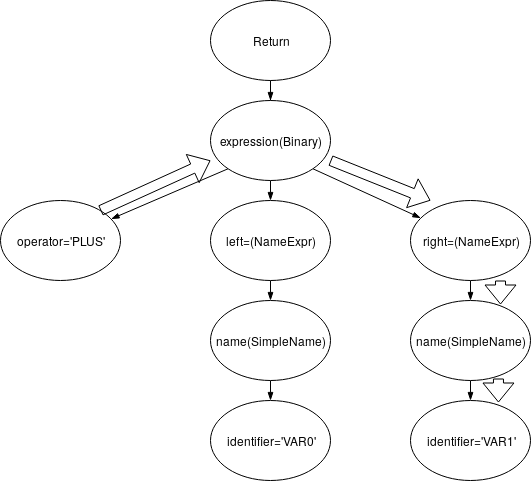
\includegraphics[width=0.4\linewidth]{img/Embedding.png}
    \caption{Example AST of Function \ref{code:examplefunction}, the example path has been superimposed with thick arrows.}
    \label{fig:exampleAST}
\end{figure}
%%%%%%%%%%%%%%%%%%%%%%%%%%%%%%%%%%%
\textbf{Dataset}
% \paragraph{Dataset}
\begin{table}[H]
    \centering
    \resizebox{\linewidth}{!}{
    \begin{tabular}{c c c c c}
    \# Methods   &  \# All tokens & \# All identifiers & \#Unique tokens & \#Unique identifiers\\
    \toprule
    588,108 & 44,378,497 & 13,779,297 & 794,711 & 794,621
    \end{tabular}}
    \caption{Statistics for code-snipets in DeepComm dataset}
    \label{tab:dataset-statistics}
\end{table}{}
%%%%%%%%%%%%%%%%%%%%%%%%%%%%%%%%%%%
\begin{figure}[H]
\centering
\subfloat[Full Distribution]{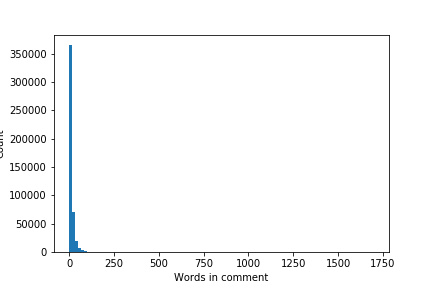
\includegraphics{img/distr.png}} 
\subfloat[\<40 words in comments]{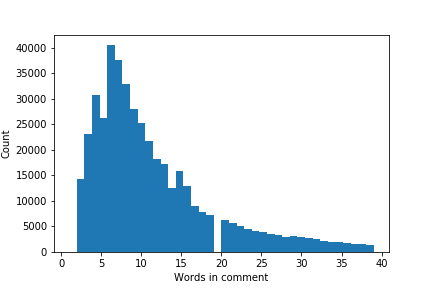
\includegraphics{img/zoomedInLength.png}}
\caption{Dataset distribution of target comment lengths.} 
\label{fig:data_dist} 
\end{figure}
%%%%%%%%%%%%%%%%%%%%%%%%%%%%%%%%%%%

% \paragraph{Encoding}
% \begin{figure}[H]
%     \centering
%     \includegraphics[width =0.8\linewidth]{Encoder(1).png}
%     \caption{Graphic representation of Encoder, $Encode(x) = \sum_{s\in x} E^{\text{subtokens}}_s$}
%     \label{fig:encoder}
% \end{figure}{}
% \paragraph{Decoding}



% \paragraph{Dataset}


\paragraph{Training}
\begin{itemize}
    \item Setup
    \begin{itemize}
        % \item Cross-entropy loss with a Nesterov momentum of 0.95.
        \item Learning rate 0.01 with 0.05 decay every epoch.
        \item Embeddings size: 128, Encoder size: 256, Decoder size: 640, Batch size: 128.
        \item Trained for 100 epochs. Early stopping if no improvement for 10 epochs. 
    \end{itemize}.  
    \item Method - 1: Code2Seq model with comments as target sequence.
    \item Method - 2: Same as method 1 but with variable names in ASTs.
    \item Evaluation: BLEU-4 score
\end{itemize}
\section{Results} 
%%%%%%%%%%%%%%%%%%%%%%%%%%
\begin{table}[H]
\centering
\begin{tabular}{cc}
\hline
Approaches & BLEU-4 score \\ \hline
DeepCom & 38.17 \\
Method-1 & 6.08 \\
Method-2 & 10.02 \\ \hline
\end{tabular}
\caption{Evaluation results on Java Methods}
\label{tab:bleu-table}
\end{table}
%%%%%%%%%%%%%%%%%%%%%%%%%%

%%%%%%%%%%%%%%%%%%%%%%%%%%%%%%%%%%%
\begin{figure}[H]
    \centering
    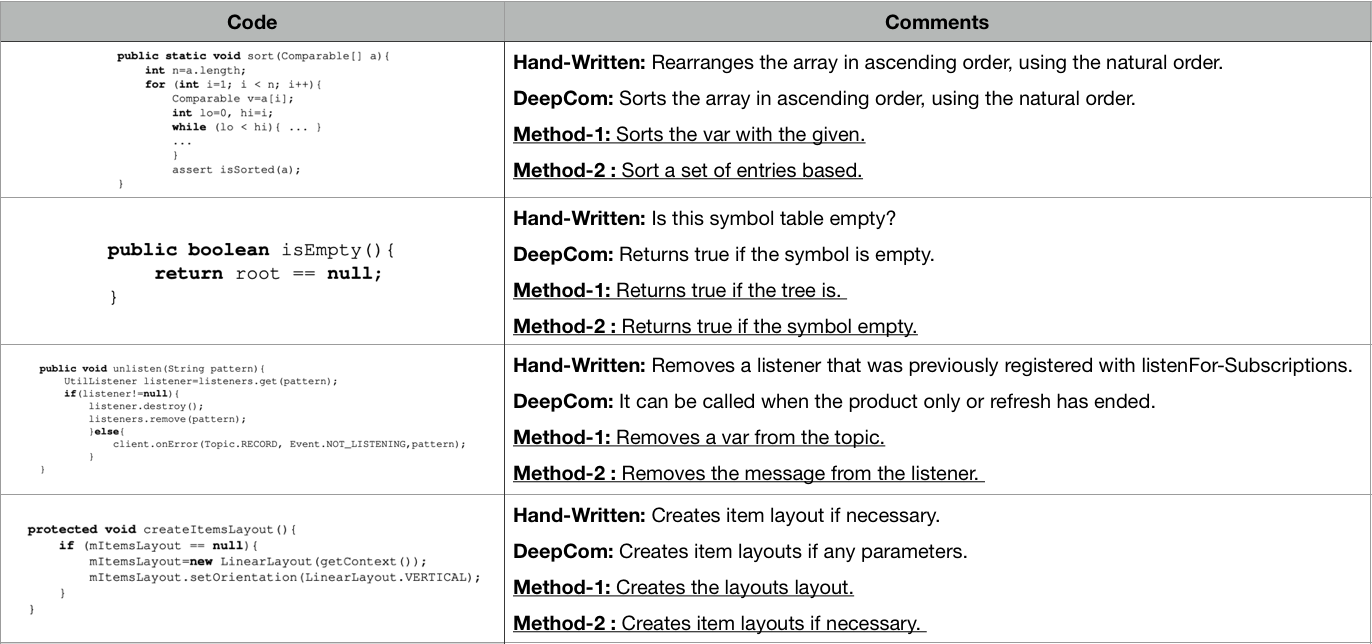
\includegraphics[width =\linewidth]{img/results_table.png}
    \caption{Comments Generated by models.}
    \label{fig:comments_gen}
\end{figure}
%%%%%%%%%%%%%%%%%%%%%%%%%%%%%%%%%%%

\section{Discussion}
\begin{itemize}
    \item Probable reasons for poor BLEU score [Table-\ref{tab:bleu-table}],
        \begin{itemize}
            \item Imbalanced distribution \ref{fig:data_dist} of target comment lengths in the dataset.
            \item Code2Seq architecture - Built to predict function names.
        \end{itemize}
    \item Performance of Method - 2, proves to be good solution to Out-of-Vocabulary problems.
    \item Model learnt the syntactic and semantic concepts from codes. [Fig - \ref{fig:comments_gen}]
    \item But, Incapable of generating longer comments (>6 words).
\end{itemize}

\section{Conclusion}
\begin{itemize}
    \item Contributions: code2seq based AutoComments, and, AST extraction to solve Out-of-Vocabulary.
    \item Future Research,
    \begin{itemize}
        \item Balanced dataset - w.r.t. target comment lengths.
        \item More experiments with decoder, for generating better comments from the learnt code semantics and syntaxes.
    \end{itemize}
\end{itemize}

\end{document}
